\documentclass[11pt, a4paper, twoside, openright]{article} %draft


\usepackage{graphicx,color}
\usepackage{amssymb, amsmath, array}
\usepackage{listings}
\usepackage{listings-golang} % import this package after listings
\usepackage{url}
\graphicspath{ {./images/} }

\lstset{ % add your own preferences
    frame=single,
    basicstyle=\ttfamily,
    keywordstyle=\color{red},
    numbers=none,   %left,
    numbersep=5pt,
    showstringspaces=false, 
    stringstyle=\color{blue},
    tabsize=4,
    language=Golang % this is it !
}

\begin{document}

% Example of title page for the projects carried out within DEDIS
% Copied from lasec 

% Simply include it in your mastex tex file: 
%        % Example of title page for the projects carried out within DEDIS
% Copied from lasec 

% Simply include it in your mastex tex file: 
%        % Example of title page for the projects carried out within DEDIS
% Copied from lasec 

% Simply include it in your mastex tex file: 
%        \input{cover}


% Updated October 2016


\newcommand{\logoepfl}[0]{
  \begin{center}
    
\includegraphics[width=4cm]{logo_epfl_coul.eps}
  \end{center}
  \vspace{0.3cm}
  \hrule
}
\newcommand{\project}[1]{
  \begin{center}
    \large{#1}
  \end{center}
  \vspace{1cm}
}
\newcommand{\department}[1]{
  \begin{center}
    \large{#1}
  \end{center}
}
\newcommand{\lab}[1]{
  \begin{center}
    \large{#1}
  \end{center}
}
\newcommand{\supervisor}[3]{
  \begin{center}
    \begin{normalsize}{
        \bf #1}\\#2\\#3
    \end{normalsize}
  \end{center}
}
\renewcommand{\author}[1]{
  \begin{center}
    \Large{#1}
  \end{center}
  \vspace{0.5cm}
}
\renewcommand{\title}[1]{
  \vspace{3cm}
  \begin{center}
    \huge{#1}
  \end{center}
  \vspace{1.7cm}
}
\renewcommand{\date}[2]{
  \begin{center}
    \normalsize{#1 #2}
  \end{center}
  \vspace{0.5cm}
}


\thispagestyle{empty}


% begin title page
  \logoepfl
  
  \title{Explore cross-platform mobile platforms}
  
  \author{Louis-Maxence Garret}
  \department{School of Computer and Communication Sciences}
  \lab{Decentralized and Distributed Systems lab}
  \project{Master Optional Project}
  
  \date{January}{2019}

  \begin{center}
    \begin{tabular}{cc}
      \begin{tabular}{p{4.0cm}}
        \supervisor{Responsible}{Prof. Bryan Ford}{EPFL / DEDIS}
      \end{tabular}&
      \begin{tabular}{p{4.0cm}}
        \supervisor{Supervisor}{Linus Gasser}{EPFL / DEDIS}
      \end{tabular}
    \end{tabular}
  \end{center}

% end title page




% Updated October 2016


\newcommand{\logoepfl}[0]{
  \begin{center}
    
\includegraphics[width=4cm]{logo_epfl_coul.eps}
  \end{center}
  \vspace{0.3cm}
  \hrule
}
\newcommand{\project}[1]{
  \begin{center}
    \large{#1}
  \end{center}
  \vspace{1cm}
}
\newcommand{\department}[1]{
  \begin{center}
    \large{#1}
  \end{center}
}
\newcommand{\lab}[1]{
  \begin{center}
    \large{#1}
  \end{center}
}
\newcommand{\supervisor}[3]{
  \begin{center}
    \begin{normalsize}{
        \bf #1}\\#2\\#3
    \end{normalsize}
  \end{center}
}
\renewcommand{\author}[1]{
  \begin{center}
    \Large{#1}
  \end{center}
  \vspace{0.5cm}
}
\renewcommand{\title}[1]{
  \vspace{3cm}
  \begin{center}
    \huge{#1}
  \end{center}
  \vspace{1.7cm}
}
\renewcommand{\date}[2]{
  \begin{center}
    \normalsize{#1 #2}
  \end{center}
  \vspace{0.5cm}
}


\thispagestyle{empty}


% begin title page
  \logoepfl
  
  \title{Explore cross-platform mobile platforms}
  
  \author{Louis-Maxence Garret}
  \department{School of Computer and Communication Sciences}
  \lab{Decentralized and Distributed Systems lab}
  \project{Master Optional Project}
  
  \date{January}{2019}

  \begin{center}
    \begin{tabular}{cc}
      \begin{tabular}{p{4.0cm}}
        \supervisor{Responsible}{Prof. Bryan Ford}{EPFL / DEDIS}
      \end{tabular}&
      \begin{tabular}{p{4.0cm}}
        \supervisor{Supervisor}{Linus Gasser}{EPFL / DEDIS}
      \end{tabular}
    \end{tabular}
  \end{center}

% end title page




% Updated October 2016


\newcommand{\logoepfl}[0]{
  \begin{center}
    
\includegraphics[width=4cm]{logo_epfl_coul.eps}
  \end{center}
  \vspace{0.3cm}
  \hrule
}
\newcommand{\project}[1]{
  \begin{center}
    \large{#1}
  \end{center}
  \vspace{1cm}
}
\newcommand{\department}[1]{
  \begin{center}
    \large{#1}
  \end{center}
}
\newcommand{\lab}[1]{
  \begin{center}
    \large{#1}
  \end{center}
}
\newcommand{\supervisor}[3]{
  \begin{center}
    \begin{normalsize}{
        \bf #1}\\#2\\#3
    \end{normalsize}
  \end{center}
}
\renewcommand{\author}[1]{
  \begin{center}
    \Large{#1}
  \end{center}
  \vspace{0.5cm}
}
\renewcommand{\title}[1]{
  \vspace{3cm}
  \begin{center}
    \huge{#1}
  \end{center}
  \vspace{1.7cm}
}
\renewcommand{\date}[2]{
  \begin{center}
    \normalsize{#1 #2}
  \end{center}
  \vspace{0.5cm}
}


\thispagestyle{empty}


% begin title page
  \logoepfl
  
  \title{Explore cross-platform mobile platforms}
  
  \author{Louis-Maxence Garret}
  \department{School of Computer and Communication Sciences}
  \lab{Decentralized and Distributed Systems lab}
  \project{Master Optional Project}
  
  \date{January}{2019}

  \begin{center}
    \begin{tabular}{cc}
      \begin{tabular}{p{4.0cm}}
        \supervisor{Responsible}{Prof. Bryan Ford}{EPFL / DEDIS}
      \end{tabular}&
      \begin{tabular}{p{4.0cm}}
        \supervisor{Supervisor}{Linus Gasser}{EPFL / DEDIS}
      \end{tabular}
    \end{tabular}
  \end{center}

% end title page


\newpage

\tableofcontents

\section{Introduction}
Distributed legder technology is gaining traction in many applications,
first and foremost in decentralized payment systems such as e.g. Bitcoin.
This adaption imposes challenges on the scalability of such systems, both in
total transaction throughput, as well as in the number of participating
processing nodes.

This report describes the implementation of OmniLedger
\cite{KokorisKogias2017OmniLedgerAS}, a scalable blockchain
with a flexible user interface. We will first describe the necessary background
in \ref{background} and discuss how OmniLedger improves on the current state of
blockchain technology.

We will also discuss some of the protocols and data structures employed by our
implementation.

Section \ref{implementation} will discuss implementation details such as how
transactions are processed, how clients interact with the service and how
access control is implemented.

Finally, section \ref{conclusion} will outline future work and conclude.

\section{Background} \label{background}
The issue of scaling blockchains has been nicely summarized in
\cite{croman2016scaling}. To give the reader some motivation and context,
we will now discuss some of the points from that paper
which are relevant to the system at hand.
The authors of \cite{croman2016scaling} differntiate between several planes,
such as e.g. the
\textit{Network Plane}, the \textit{Storage Plane} and the
\textit{Consensus Plane}. OmniLedger is mainly concerened with optimizing the
Consensus Plane.
Key issues of the Consensus Plane the authors of \cite{croman2016scaling} 
identify include:
\begin{itemize}
    \item \textbf{The consensus protocol}:
        Bitcoin's Nakamoto consensus \cite{nakamoto2008bitcoin} allows
        (theoretically) for $f$ byzantine nodes out of $2f + 1$ nodes, but a
        protocol with stronger assumptions, such as
        \textit{Practical Byzantine Fault Tolerance} (PBFT)
        \cite{castro1999practical} could be more efficient.
    \item \textbf{Improving proof-of-work protocols}:
        In the Bitcoin protocol, there is a tradeoff between consensus speed
        (and thus bandwidth) and the number of forks.
    \item \textbf{Sharding}:
        The authors suggest that splitting up the consesus protocol between
        individual shards could increase throughput.
\end{itemize}

This report describes the current implementation of \textit{OmniLedger}
\cite{KokorisKogias2017OmniLedgerAS}.
Omniledger is designed as a scalable, permissionless, sharded ledger.
The motivation for the project is to create a
decentralized ledger with the ability to "scale-out", i.e. increase throughput
linearly with the number of nodes.
To do so, Omniledger captures the ideas from \cite{croman2016scaling} listed
above. We will now go over each of them, and discussing how OmniLedger makes
use of it to improve latency, throughput and scalability.

\subsection{The Consensus Protocol}
OmniLedger uses ByzCoin \cite{Kokoris-Kogias:220209} as a consesnus protocol.
In ByzCoin, the nodes decide collectively on one single chain, no forks
occur.
ByzCoin is a byzantine fault tolerant consesus protocol, whcih guarantees
safety and liveness for up to $f$ byzantine nodes out of $3f + 2$ total nodes.
When a block is to be added to the blockchain, a consensus round is run in
order to vote on whether to accept or reject the block.
Due to this mechanism, no forks can occur in the blockchain. Therefore, no work
which is put in the validation of blocks is ever lost, as would be the case if
a fork occured and one of the branches had to be pruned.

ByzCoin is based on PBFT \cite{castro1999practical}, but reduces the
communication complexity from $O(n^2)$ to $O(\log n)$ by using a tree based
collective signing protocol \cite{Syta:221010}.
The node at the root of this tree is the one which initializes the collective
signing protocol. We will refer to this particular node as the \textit{leader}
in future occurences.\\

\begin{figure}[htb!]
    \centering
    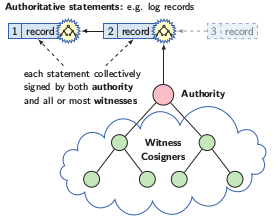
\includegraphics{byzcoin.png}
    \caption{ByzCoin's collective signing protocol: The nodes are organized in
    a tree structure and collectively sign each block (copied from
    \cite{Syta:221010}).}
\end{figure}


\subsection{The Proof-of-Work Protocol}
In order to establish Sybil attack resistant identities for ByzCoin's
consensus group, an identity blockchain, separate from the data holding
blockchain is employed:
When a miner finds a new block of this chain, she receives a \textit{consensus
group share}, which gives her voting power on data holding blocks until the
next $w$ blocks of the identity blockchain have been mined.
This decouples the Proof-of-Work from the verification of transactions,
allowing for a lower transaction processing latency.\\

\subsection{Sharding}
In order to take load off of individual nodes as well as reduce consesnus group
size (which in turn reduces consensus latency), OmniLedger employs sharding.
This means, that each validoator is only repsonsible for a subset of the data,
namely its shard.

Letting nodes choose the shard they are responsible for might allow an
attacker to focus on one single shard and control it. Therefore, nodes must be
assigned to shards in a secure, random way.
In order to assign validators to shards, OmniLedger uses RandHound
\cite{syta2017randhound}.
RandHound is a scalable public randomness generation protocol.
It provides publicly-verifiable randomness which can neither be biased nor
predicted by any involved party except with negligible probability, as long as
there are at most $f$ malicious nodes out of $3f + 1$ total nodes.

The protocol is designed as a client/server model, where a client requests
randomness from a set of servers (nodes).
The protocol works roughly as follows:
\begin{itemize}
    \item The client allocates the servers to disjoint groups.
        The members of a given group will have to set up a shared secret.
        Splitting the servers up into groups instead of having one global
        group reduces the communication complexity.
    \item Each server chooses a secret random value. The servers of a group
        then create a shared secret based on all the random values of the
        group.
    \item Each server then sends his encrypted share of the secret to the
        client, who then chooses a subset of the servers and submits this
        selection to the nodes for collective signing \cite{Syta:221010}.
    \item Subsequently, the servers send their unencrypted shares of the
        secret to the client who combines them to obtain the final random
        output.
\end{itemize}

This is only a quick overview over RandHound, for more details, consider
\cite{syta2017randhound}.\\

OmniLedger supports cross shard transactions, i.e. transactions which touch
data in more than one shard. Since one shard might allow his part of a
transaction while the other does not, such
transactions must be processed atomically. Otherwise the shards could end up
in an inconsistent state. In a payment system, this means that funds could
be locked forever.
Atomicity is acheived by \textit{Atomix} \cite{KokorisKogias2017OmniLedgerAS},
an atomic cross-shard commit protocol. 
Atomix is a client driven protocol, where the client first locks all the
resources the transaction touches. If a shard does not allow the transaction
the client will not be able to obtain the corresponding lock.
If the client could obtain all locks, he can subsequently unlock the resources
and commit the transaction. Otherwise he unlocks to abort it.
Since a shard is collectively honest and does not fail (this is acheived by
Randhound, see above), this protocol is sufficient to provide the desired
functionality.\\

\subsection{Skipchain: The Underlying Data Structure}
While not specified in \cite{KokorisKogias2017OmniLedgerAS}, the implementation
of OmniLedger uses the \textit{skipchain} \cite{nikitin2017chainiac}:
A skipchain is a blockchain which contains cryptographically signed forward
links:
In addition to the backwards pointing hash of the previous block, as known from
e.g. Bitcoin \cite{nakamoto2008bitcoin}, each block also contains pointers to 
future blocks.

\begin{figure}[htb!]
    \centering
    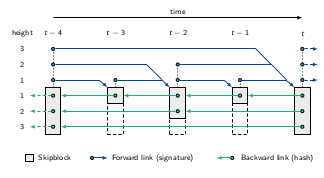
\includegraphics[scale=0.9]{skipchain.png}
    \caption{The skipchain: Both backward and forward links can span multiple
    hops, which allows a client to efficiently traverse the chain
    (copied from \cite{nikitin2017chainiac}).}
\end{figure}

These links enable a client to securely traverse time in forward as well as
in backward direction. Since forward links may point to blocks several
positions ahead, blocks can be skipped when traversing the skipchain.
This allows for more efficient traversal, which is important for clients which
have not caught up with the skipchain's state in a long time.
Since forward links point to future blocks, they can not be added at block
creation time - the block they should point to does not yet exist.
Therefore, they are added only once their target block exists and then 
cryptographically signed by the set of nodes that created the original block.
This requires the corresponding nodes to stay live until all future blocks
for which they have to sign forward links have been created.

Now we have seen how OmniLedger aims to improve current blockchain
implementations. The paper however focuses mainly on the protocols needed for
these improvements and does not provide further detail on how clients interact
with the system or how transactions are applied to the system's state.
Therefore, the next section will put its focus on these aspects of the
implementaion.


\section{Implementation} \label{implementation}
We will now discuss the current state of the OmniLedger implementation.
The system is developed in the \textit{Go} language \cite{golang}.\\

In section \ref{background}, several building blocks which improve the
scalability of blockchains have been described. Some of these have already
been implemented in the \textit{Cothority framework} \cite{coth},
notably ByzCoin in the package \textit{ByzCoinX} and the skipchain. The
skipchain implementation already uses ByzCoinX, therefore our OmniLedger
implementaion is built on top of it.

Currently, not all of the features described in section \ref{background} are
implemented, but they are planned to be in the future.
For now, the only feature from section \ref{background} present in the
implementation is the consensus protocol: ByzCoinX.
Furthermore, it should be noted that view changes in case the leader fails are
currently not implemented in the skipchain we use.

For the moment, in contrast to the system described
in \cite{KokorisKogias2017OmniLedgerAS}, the implementation operates as a
permissioned blockchain. This means that the processing nodes of a skipchain
must be known when it is initiated.\\
%TODO: Anything else?

Having discussed the motivation and relevant background in \ref{background},
this section will now focus on how clients interact with the system
and how transactions are processed.\\

First, a brief overview over the implementation's working principles will be
given.  We will then discuss the service's components and how transactions are
processed in more detail.
Finally, we will describe the messages the clients can use to interact with
OmniLedger.
%TODO: Explain why we use this approach.

From now on, the name \textit{OmniLedger} will refer to the implementation
described in this section. If we refer to the paper
\cite{KokorisKogias2017OmniLedgerAS}, we will do this explicitly.


\subsection{Overview} \label{overview}
OmniLedger is implemented as a service accepting requests from clients.
It maintains several independent skipchains, each storing its own state.
The nodes of each skipchain are organized in a static tree, the leader at the
root. We will refer to the nodes who are not the leader as \textit{validators}.

The leader accepts clients' requests, queues them and periodically issues
blocks, containing the transactions which have been queued since the last
block.
The validators must then find consensus on whether or not they accept the
proposed block via ByzCoinX. If the block is accepted, its transactions will be
applied.

A client's transaction is only accepted if the client can prove that he has the
right to perform this transaction.
The access right control is implemented via \textit{Darcs}, which
is short for distributed access rights control.
These rights are part of the service's state itself and can also be evolved by
the corresponding transactions.

Before we start discussing how OmniLedger processes transactions, we need first
to discuss darcs a little bit, in order to understand how access control is
implemented.\\

A darc is a structure which contains rules, a mapping from actions
to expressions.
An action can be performed if and only if the corresponding expression is
satisfied. An expression is a formula over identities which
contains conjunctions and disjunctions. An identity can either be an Ed25519
public key, an X509EC public key or a darc itself.
Having a darc as an identity allows to delegate access rights to groups of
entities rather than just share a private key.
An expression is satisfied if a set of signatures is provided, which satifies
the formula.\\
The darc package provides the following example in its documentation:
Assume an expression of the form $(a \land b) \lor (c \land d)$.
Then, the expression is satisfied if and only if
either both signatures of the identities $a$ and $b$ are provided, or both
signatures of $c$ and $d$ are provided.
Given the corresponding access rights, a darc can be evolved, meaning that
rules (i.e. action-expression mappings) can be added, modified, or removed.
Evolving a darc will create a copy of it which contains a reference to all the
previous versions of it.
This allows a client to later correctly verify the evolution of the darc,
by checking the signatures provided at each evolution step.\\

OmniLedger stores all of its state in a Merkle-tree based data structre.
This allows the service to provide cryptographic proofs about the
presence or absence of a given item in its state. Any client holding the
Merkle-root of the tree can then verify these proofs.

To allow clients to obtain the Merkle-root in a secure fashion, it is stored in
the block's header, which will also contain the hashes of all transactions and
the resulting state modifications applied with that block.

% TODO: Block structure
\begin{figure}[htb!]
    \centering
    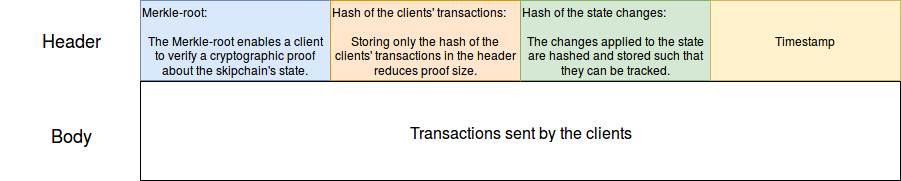
\includegraphics[scale=0.40]{block.png}
    \caption{The structure of a skipblock. Only the data in the header is
    needed to validate the state of a skipchain.}
    \label{f:block}
\end{figure}

Figure \ref{f:block} shows the structure of OmniLedger's skipblock. We will
discuss the content of the depicted fields in the follwoing.
Note that the figure does not display any information about forward links or
other data belonging to the skipchain implementation, since OmniLedger does not
handle these.

Now that an overview over the system has been established, we will discuss the
individual components needed to store state and process transaction in more
detail.

\newpage
\subsection{Components}
The OmniLedger service's components are grouped together in the type
\texttt{Service}.

\begin{lstlisting}[caption={The structure of the OmniLedger service.},captionpos=b]
type Service struct {
	// We need to embed the ServiceProcessor,
    // so that incoming messages are correctly
    // handled.
	*onet.ServiceProcessor
	// collections cannot be stored,
    // so they will be re-created whenever 
	// the service reloads.
	collectionDB map[string]*collectionDB

	// wokersMu protects access to queueWorkers
	workersMu sync.Mutex
	// queueWorkers is a map that points to
    // channels that handle queueing and
	// starting of new blocks.
	queueWorkers map[string]chan ClientTransaction

	// CloseQueues is closed when the queues
    // should stop - this is mostly for
	// testing and there should be a better
    // way to clean up services for testing...
	CloseQueues chan bool
	// contracts map kinds to kind specific
    // verification functions
	contracts map[string]OmniLedgerContract
	// propagate the new transactions
	propagateTransactions messaging.PropagationFunc

	storage *storage

	createSkipChainMut sync.Mutex
}
\end{lstlisting}

In short, communication is handeled by the embedded
\texttt{onet.ServiceProcessor}, state is stored in the \texttt{collectionDB},
\texttt{queueWorkers} are channels
used to communicate with worker functions which queue requests and create
blocks, each one associated to a given skipchain. \texttt{CloseQueues} is used
to terminate the worker functions, and \texttt{workersMu} is used to protect 
\texttt{queueWorkers} from concurrent accesses.
The variable \texttt{contracts} associates to each kind of state an
\texttt{OmniLedgerContract}, which is essentially a function which takes state,
a so called \texttt{Instruction} and a slice of \texttt{coin}s and returns
all the changes it has applied to the state, as well as a slice of remaining
\texttt{coins}. The \texttt{coin}s can be used to limit the amount of
instructions a client can execute.

We will now discuss the most important components and some of their interfaces
in more detail. For further information, we would like to refer you to the
corresponding repository \cite{omni}.

\subsubsection{State Storage: Collections}
At the heart of the service lies the type \texttt{Collection}. A collection is
a Merkle tree based data structure, which allowes to store key-value
associations in the form of \texttt{byte} slices and can issue cryptographic
profs of the presence or absence of a key-value pair. It allows to store data
on an untrusted server while still having proofs about it's exact state.
In the implementation, we use the wrapper \texttt{collectionDB}, which allows
us to use a \textit{BoltDB} \cite{bbolt} to store the state.
The type \texttt{collectionDB} exposes \texttt{Add}, \texttt{Set} and
\texttt{Delete} methods, which allow to add new key-value pairs, set the value
for a given key or remove a key-value pair from the collection, respectively.
%TODO: GetProof

\subsubsection{Processing Transactions with Contracts}
The OmniLedger service uses the \texttt{collectionDB} to store state associated
with so called \texttt{OmniLedgerContract}s. These contracts define how clients
can interact with the service. They are responsible for applying the deciding
whether the transactions in a lock are valid or not and thus whether the block
should be accepted or not.

Clients send transactions to the service, (see type \texttt{ClientTransaction})
which contain insdivitual instrucions (see the type \texttt{Instruction}).
An instruction contains one of three actions:
\texttt{Spawn}, \texttt{Invoke} and \texttt{Delete}.
These actions allow to initiate a contract with a specified initial state or 
modify or remove the state associated with a contract. 
The spawn and invoke instructions can also contain arguments
format which the contract can access.
Additionally -among others-, an instruction contains an
\texttt{ObjectID} which
works as a key for the collection in order to identify the state to
be modified or deleted, or as a definition of a new intial state's key.
Additionally, the \texttt{ObjectID} contains a \texttt{DarcID}, which in turn
points to the darc which is responsible for the access rights to this object.
Furthermore, an \texttt{Instruction} contains a slice of darc signatures, the
use of which will be discussed below.

Each value stored in the collection contains a \texttt{ContractID}.
This ID is a key for the service's \texttt{contracts} map,
which contains \texttt{OmniLedgerContract}s as values.
These contracts have the type
\texttt{func(cdb collection.Collection, tx Instruction, c []Coin) ([]StateChange, []Coin, error)}.
Contracts specify how the Instructions are to be interpreted by
the service. Since the interpretation of \texttt{Instruction}s depends on the
state of the collection, a contract takes a reference to it as an
input parameter. Additionally, \texttt{coin}s can be required to limit the
number of instructions a client can execute.
The \texttt{ContractID} and the state of the contract is stored in the
collection, accessible via the key \texttt{ObjectID} contained in
the interpreted instruction.
When a block is proposed to the validators, they iterate through each
transaction in it and apply the corresponding contract to each instruction.

In order to ensure that only clients with the corresponding access rights
interact with a given object, the contracts can check the darc signatures in
the instruction against the darc pointed to by the \texttt{ObjectID}.
If the contract does not output an error, the instruction is considered valid.
A transaction is valid if and only if all its instructions are
valid. This prevents the service from partially applying
transactions, which might otherwise have effects which the client did not
expect.

For valid transactions, the contract outputs a slice of
state changes (see the type \texttt{StateChange}).
A state change contains a \texttt{StateAction},
one of \texttt{Create}, \texttt{Update} or \texttt{Remove}. These
state changes can only be created from \texttt{Spawn}, \texttt{Invoke}
and \texttt{Delete} instructions, respectively.
The state change also contains a \texttt{ContractID}, an
\texttt{ObjectID} and a value. For the \texttt{Create}/\texttt{Update}
action, the value with the key specified in the \texttt{ObjectID} is
inserted/updated with the value and the \texttt{ContractID}.
For the \texttt{Delete} instruction, this data is ignored, since a
\texttt{Delete} instruction simply removes the corresponding key-value pair.

The advantage of translating instructions to state changes, is that it provides
a more flexible interface for the clients which is easier to extend. One could
e.g. also imagine instructions which are not translated to single state
changes, but to a sequence.\\

We have now seen how clients sent transactions to OmniLedger and how the
validity of blocks is ensured. The corresponding state changes are then only
applied when the block has been accepted.

Having seen how a transaction is processed from the client to the collection,
we will now discuss how the queueing of transactions at the leader is
implemented.

\subsection{Worker Functions}
In order to reduce the amount of blocks on which the system has to vote,
and thus improve throughput (in terms of transactions per second),
transactions are queued at the leader.
This is implemented by having one Goroutine per skipchain which listens on a
channel for new incoming requests and creates a block containing all queued
requests periodically. The frequency of blocks can be specified by the client
when the skipchain is created. The channels to communicate with these worker
functions are accessible through the \texttt{queueWorkers}-map via the
corresponding skipchain's \texttt{SkipChainID}.\\

We have now seen how blocks are created by the leader and how contracts are
used to validate transactions and thus vote on proposed blocks.\\

We will now discuss what messages the client can use to interact with the
service and how they are handled by OmniLedger.

\subsection{Messages}

The OmniLedger service accepts the following messages from clients:\\

\subsubsection{Create the Genesis Block of a New Skipchain}

The message \texttt{CreateGenesisBlock} creates a new skipchain at the service
which will be maintained by the nodes specified in the \texttt{Roster}
variable.
A genesis darc is stored in the genesis block, and in order to write to this
skipchain subsequently,
a client must provide the signature of that darc. Thus, the entire
configuration of this new skipchain can be found in it's genesis block.

\begin{lstlisting}[caption={The structure of the \texttt{CreateGenesisBlock} message.},captionpos=b]
// CreateGenesisBlock asks the service
// to set up a new skipchain.
type CreateGenesisBlock struct {
	// Version of the protocol
	Version Version
	// Roster defines which nodes
    // participate in the skipchain.
	Roster onet.Roster
	// GenesisDarc defines who is
    // allowed to write to this skipchain.
	GenesisDarc darc.Darc
	// BlockInterval in int64.
	BlockInterval time.Duration
}
\end{lstlisting}

\newpage
The reply a client receives to this request (if no error occurred at the
service while handling the request)
is of the type \texttt{CreateGenesisBlockResponse}:

\begin{lstlisting}[caption={The structure of the \texttt{CreateGenesisBlockResponse} message.},captionpos=b]
// CreateGenesisBlockResponse holds the
// genesis-block of the new skipchain.
type CreateGenesisBlockResponse struct {
	// Version of the protocol
	Version Version
	// Skipblock of the created skipchain
    // or empty if there was an error.
	Skipblock *skipchain.SkipBlock
}
\end{lstlisting}

The \texttt{CreateGenesisBlock} request is handled by the service's
method \texttt{CreateGenesisBlock}. This method makes sure that the
\texttt{GenesisDarc} has the correct format, creates the genesis
\texttt{Transaction} and uses it to create a new block which is then proposed
to the other nodes to sign them via ByzCoinX protocol.
Additionally, an asynchronous worker function corresponding to this
new skipchain is created, which will queue requests
and create blocks as specified in the \texttt{BlockInterval} field of the
request.
The worker function is implemented as a Goroutine which listens to requests
on a channel stored in a \texttt{map} and has the corresponding
\texttt{SkipchainID} as key.\\

\subsubsection{Add a New Transaction}
A client can request the service to execute a transaction by sending a message
of the type \texttt{AddTxRequest}:

\begin{lstlisting}[caption={The structure of the \texttt{AddTxRequest} message.},captionpos=b]
// AddTxRequest requests to apply
// a new transaction to the ledger.
type AddTxRequest struct {
	// Version of the protocol
	Version Version
	// SkipchainID is the hash of the first skipblock
	SkipchainID skipchain.SkipBlockID
	// Transaction to be applied to the kv-store
	Transaction ClientTransaction
}
\end{lstlisting}

This message contains the transaction to be executed.
The service handles the instructions with the
\texttt{AddTransaction} method, which checks that the corresponding skipchain
exists and then writes the \texttt{Transaction} to the corresponding channel.
The worker listening on the channel then takes care of creating the
corresponding block and propose it to the validators, which will then vote on
it.

Since the block is not necessarily issued directly after the request has been
processed by the leader, the reply to this type of request is just an
\textit{ack}, containing the version of the running service.



\subsubsection{Get a Proof About the Collection's State}

As described in subsection \ref{overview}, clients can obtain proofs about the
collection's state. This is done by sending a message of the type
\texttt{GetProof} to the service. The service will handle this request by
creating a proof of the presence or absence of the value associated with
\texttt{Key}. 

\begin{lstlisting}[caption={The structure of a \texttt{GetProof} message.},captionpos=b]
type GetProof struct {
	// Version of the protocol
	Version Version
	// Key is the key we want to look up
	Key []byte
	// ID is any block that is known to
    // us in the skipchain, can be the genesis
	// block or any later block. The proof
    // returned will be starting at this block.
	ID skipchain.SkipBlockID
}
\end{lstlisting}

To obtain a verifiable proof, the client sends the ID of the last skipblock of
the corresponding skipchain he knows. The service then replies by sending
a structure containing an inclusion  proof from the collection in its current
state, the most recent block of the skipchain as well as the cryptographically
singed forward links from the client's last known block to the latest
skipblock. With this information, the client can now retrieve the Merkle-root
of the collection in its current state from the last skipblock and verify the
inclusion proof of the collection. Since the forward links from the last known
block to the latest block are signed, the client can rest assured that the
Merkle-root he retrieves from this block is genuine.

This section has described how OmniLedger's implementation processes clients'
transactions and how clients can interact with the system. 

The next section will offer a conclusion about the work done so far and briefly
talk about future work.

\section{Conclusion and Future Work} \label{conclusion}

This report has presented the implementation of OmniLedger, as well as the
necessary background on how this system fits into current blockchain technology
and how it seeks to improve the state of said technology.

It has been shown how OmniLedger implements contracts to control how state is
modified, and what language (i.e. transactions) is used to interact with it.
Additionally we have seen how darcs can be used to have access rights which can
be delegated, and where a specific combination of signatures can be required.

We have, however not seen any applications running on top of OmniLedger, in
part because this would be beyond the scope of this report, but also since
such applications -at the time of writing- have not yet been implemented or
ported to OmniLedger.

However, several applications are planned to be implemented on top of
OmniLedger. One example are \textit{Onchain-secrets} \cite{kokorishidden},
which would enable a
blockchain to securely store secrets which are only accessible to clients
which can provide the corresponding credentials. This could be implemented by
having nodes holding the secret in an encrypted form and sending the
corresponding key to the clients provided the correct credentials, log the
access in the skipchain and then re-encrypt the secret with a new key.

Another application, which is currently implemented in the Cothority
Framework, but is planned to be ported to Omniledger is
\textit{Proof of Personhood} \cite{ford2007pseudonym}.
Proof of Personhood (PoP) anonymously links a
cryptographic token to a physical person, such that no person can have more
than one token. This can be achieved by organizing parties with physical
attendees who each deposit a public key, mutually verify that each attendee is
an actual person, and then collectively sign the set of key. 
The results and proceedings of such parties could be stored on OmniLedger.

We hope that OmniLedger can be used as a flexible platform to implement a wide
variety of services.

\appendix
\section{Installation}
The OmniLedger implementation is written in Go \cite{golang}. Therefore, an
installation of Go should be present on the host where OmniLedger is to be
installed. Note that the version of Go should not be older than 1.9.
To install Go, follow the instructions in \cite{goinstall}.
Furthermore, \texttt{git} should be installed on the host.

Once the Go installation is up and running, create the directory\\
\texttt{\$GOPATH/src/github.com/dedis}
and \texttt{cd} into it.

Now type \texttt{go get github.com/dedis/student\_18\_omniledger}.
This will clone the repository into your current directory.
In order to get the dependencies needed to build the project, run
\texttt{go get ./...} in the projects root directory.
This will automatically download all the dependencies declared in the source
code.\\

The OmniLedger service itself does not provide any \texttt{main} method, but
tests can be run from the repository's root directory with \texttt{make test}.


\bibliographystyle{plain}
\bibliography{references}
\end{document}
